\documentclass[11pt, a4paper, oneside]{article}

% hifenização e outras especificações para português
\usepackage[portuguese]{babel}

% hiperligações
\usepackage{hyperref}
\hypersetup{colorlinks=true, urlcolor=blue, linkcolor=black}

% escrever acentos e coisas do género sem que o latex se desoriente
\usepackage[utf8]{inputenc}

% para ter imagens, depois define a directoria de imagens
\usepackage{graphicx}
\graphicspath{{./imagens/}}

\usepackage[labelformat=simple]{caption}
\usepackage[labelformat=empty]{subcaption}

% para ter a informação de quantas páginas tem o documento
\usepackage{lastpage}

% definir o cabeçalho e rodapé
\usepackage{fancyhdr}
\pagestyle{fancy}
\fancyhead[L]{\small{Processamento da Wikipédia}}
\fancyhead[R]{\small{Processamento de Linguagens}}

% ter enumerações alinhadas
\usepackage{enumitem}

% escrever algoritmos
\usepackage[algoruled]{algorithm2e}

% mais cores predefinidas
\usepackage[usenames,dvipsnames]{color}

% definir comandos especiais
\newcommand\doubleplus{+\kern-1.3ex+\kern0.8ex} %

\newcommand{\todo}[1] {\textcolor{BrickRed}{\begin{quote}#1\end{quote}}}



%%%%%%%%%%%%%%%%%%%%%%%%%%%%%%%%%%%%%%%%%%%%%%
%% inicio do documento
\begin{document}
\title{Processamento da Wikipédia\\
\begin{normalsize}
Variante 1
\end{normalsize}}
\date{\today\\Universidade do Minho}
\author{
  Bruno Ferreira\\
  {\small A61055}\\
  \and
  Cláudia Oliveira\\
  {\small A60987}\\
  \and
  Vanessa Campos\\
  {\small A-----}\\
}

\maketitle
%\begin{abstract}
%\begin{center}
%  Lorem Ipsum
%\end{center}
%\end{abstract}
\newpage

\tableofcontents
\listoffigures 

\newpage
\section{Introdução}



\newpage
\section{Section}

Lorem ipsum dolor sit amet, consectetur adipiscing elit. Proin cursus vitae augue eu pulvinar. Fusce vulputate felis non gravida imperdiet. Duis laoreet erat a odio viverra, quis pharetra eros aliquam. Donec orci mi, varius at tellus sed, dignissim euismod leo. Nulla semper convallis est, ut accumsan orci. Mauris vitae turpis sodales felis consectetur elementum ac sed lacus. Praesent gravida lacus sit amet massa ornare condimentum. Aliquam lectus quam, interdum in urna ut, euismod vulputate ligula. Vivamus nibh odio, volutpat id ligula nec, mattis pulvinar lacus. Ut nibh lectus, tristique nec porta sed, convallis sit amet massa. Praesent non sem ipsum. Nam varius blandit massa sed vulputate. Lorem ipsum dolor sit amet, consectetur adipiscing elit. Cras sit amet ornare urna.

Phasellus consequat elit sit amet ultrices eleifend. Phasellus malesuada semper quam, malesuada malesuada tellus ultricies id. Quisque et scelerisque lectus. Suspendisse rutrum dui quis volutpat volutpat. Maecenas quis molestie massa. Suspendisse aliquam malesuada neque eget accumsan. Nam cursus bibendum tortor vehicula iaculis. Sed tincidunt volutpat dui. Nullam dapibus nulla nulla.

\subsection{Subsection}

Lorem ipsum dolor sit amet, consectetur adipiscing elit. Vestibulum id sem vitae velit porta imperdiet ut vitae nunc. Fusce vehicula pharetra dolor, id aliquet ligula facilisis in. Nulla at tellus sapien. Nullam eu diam nec nisi placerat pharetra. Ut a lacus ut augue varius semper. Nulla facilisi. Ut imperdiet, ligula vitae pharetra congue, purus augue semper nisl, sed suscipit eros sem in orci. Vestibulum erat quam, sollicitudin et molestie non, faucibus eu ante. Aliquam egestas ac elit ut rutrum. Mauris pulvinar eleifend eros. Suspendisse euismod euismod elementum.

\subsubsection{subsubsection}

Suspendisse scelerisque nec odio sed rhoncus. Mauris luctus ullamcorper urna. Class aptent taciti sociosqu ad litora torquent per conubia nostra, per inceptos himenaeos. Sed scelerisque porta massa id scelerisque. Etiam pharetra porta sapien ac rhoncus. Curabitur non purus aliquet, porttitor lorem dictum, viverra urna. Quisque diam erat, mattis sit amet purus ac, dictum eleifend libero. Maecenas luctus pellentesque mollis. Duis molestie pellentesque turpis a porttitor.

\newpage
\section{WANTED: DEAD OR ALIVE}
\begin{figure}[h!]
  \centering
    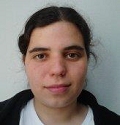
\includegraphics[width=0.6\textwidth]{107}
  \caption[Descrição no titulo]{Descrição abaixo da imagem}
\end{figure}
\newpage

\todo{pode-se utilizar esta tag para chamar a atenção para coisas que é preciso fazer antes de entregar o relatório}

\newpage
\section{Elementos do Grupo}
\begin{figure}[h!]
\centering
\begin{subfigure}{.33\textwidth}
  \centering
  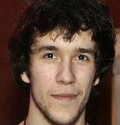
\includegraphics[width=0.8\linewidth]{60}
  \caption{Bruno Ferreira  }
\end{subfigure}%
\begin{subfigure}{.33\textwidth}
  \centering
  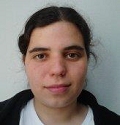
\includegraphics[width=0.8\linewidth]{107}
  \caption{Cláudia Oliveira}
\end{subfigure}%
\begin{subfigure}{.33\textwidth}
  \centering
  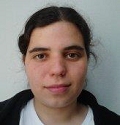
\includegraphics[width=0.8\linewidth]{107}
  \caption{Vanessa Campos}
\end{subfigure}%
\end{figure}


\end{document}